\documentclass[standalone]

\usepackage{tikz}
    \usetikzlibrary{%
        arrows.meta,
        decorations.pathreplacing,
        decorations.text,
        patterns,
        shapes.arrows,
        shapes.geometric
    }

\tikzstyle{every picture} += [remember picture]
\tikzstyle{na} = [baseline=-.5ex]

\tikzset{%
    fullcolumn/.pic={%
        code{%
            \draw[line width=1pt]
                (0, 0) --
                ++(0, #1*10pt) --
                ++(-2cm, 0) --
                ++(0, -#1*10pt) -- 
                (0, 0);
            \foreach \val in {0, ..., #1}{%
                \draw[rotate=90]
                    ([xshift=-\val*10pt] #1*10pt, 2cm) -- ++(0, -2cm);
            };
        }
    }
}

\begin{document}

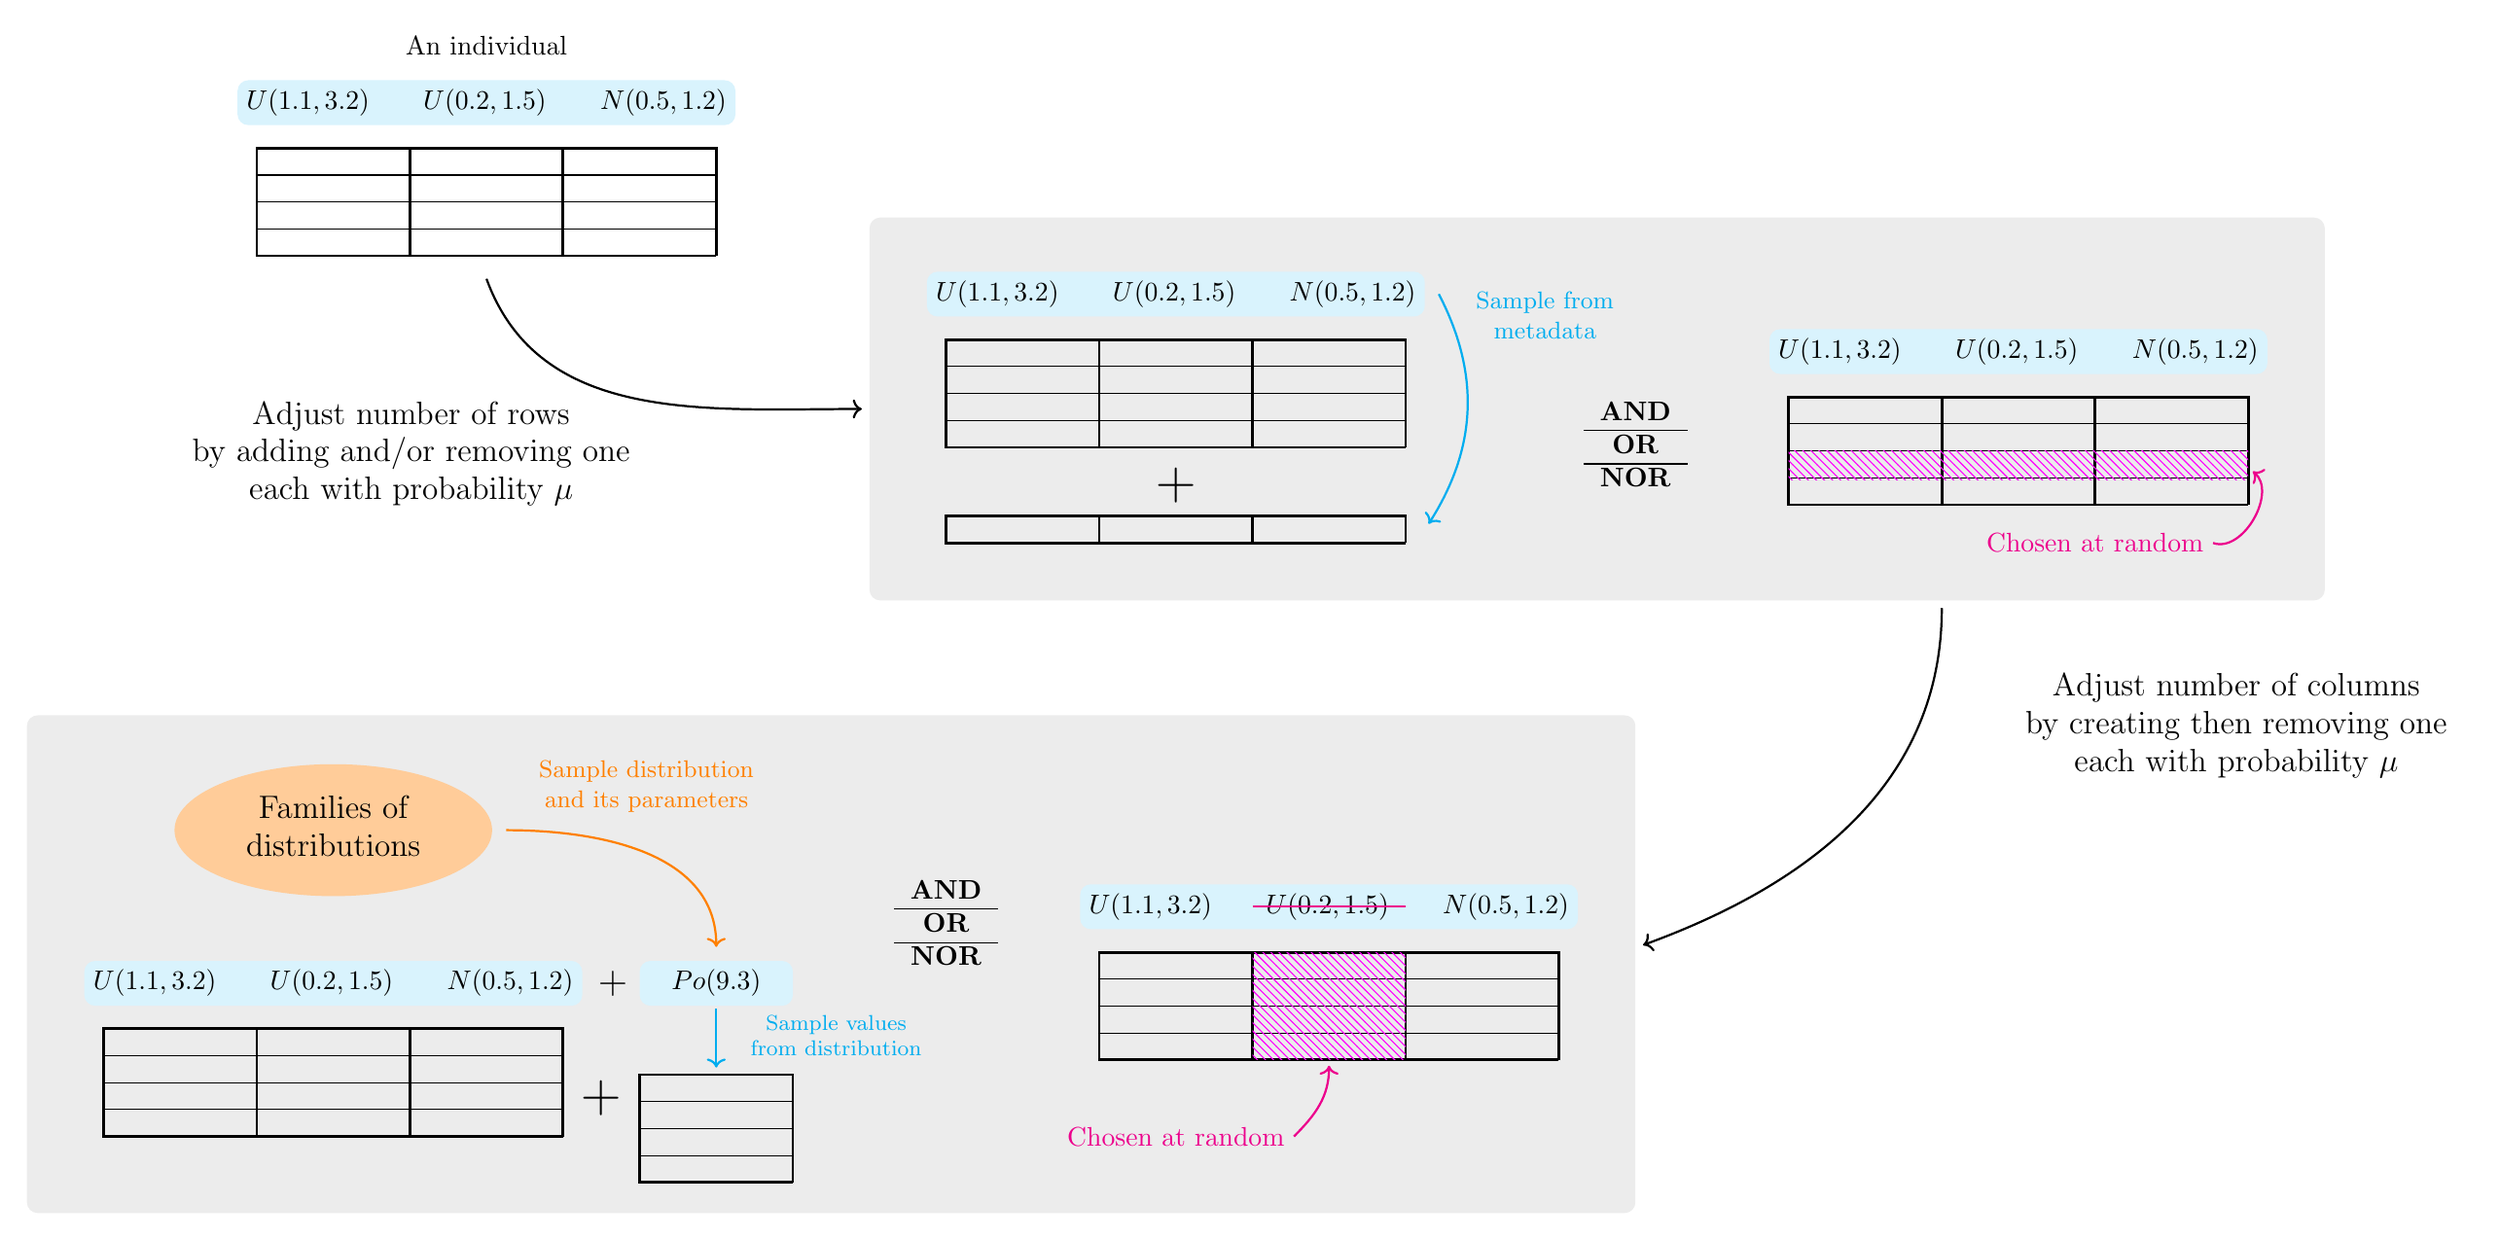
\begin{tikzpicture}

    % Individual
    \path (0, 1.5) pic {fullcolumn=4}
          (2, 1.5) pic {fullcolumn=4}
          (4, 1.5) pic {fullcolumn=4};

    \node (individual) at (1, 1.5) {};
    \node[fill=cyan!15, minimum width=6cm, rounded corners] at (1, 3.5)
        {\(U(1.1, 3.2) \qquad U(0.2, 1.5) \qquad N(0.5, 1.2)\)};
    \node at (1, 4.25) {An individual};


    %%% Adjust length
    \fill[gray!15, rounded corners] (6, -3) rectangle (25, 2);
    \draw[->, black, thick]
        ([yshift=-5pt] individual.south)
        to [out=290, in=180] node[left=50pt, below=10pt, pos=0.25] {\large%
            \begin{tabular}{c}
                Adjust number of rows\\
                by adding and/or removing one\\
                each with probability \(\mu\)
            \end{tabular}
        } (5.9, -0.5);

    % Row addition
    \path (9, -1) pic {fullcolumn=4}
          (11, -1) pic {fullcolumn=4}
          (13, -1) pic {fullcolumn=4};
 
    \node[fill=cyan!15, minimum width=6cm, rounded corners] (r-info) at (10, 1)
        {\(U(1.1, 3.2) \qquad U(0.2, 1.5) \qquad N(0.5, 1.2)\)};

    \path (9, -2.25) pic {fullcolumn=1}
          (11, -2.25) pic {fullcolumn=1}
          (13, -2.25) pic {fullcolumn=1};

    \node (new-row) at (13, -2) {};
    \node (row-plus) at (10, -1.5) {\huge\(+\)};

    \draw[->, cyan, thick]
        ([xshift=5pt] r-info.east)
        to [bend left=30] node[right, pos=0.1] {\small%
            \begin{tabular}{c}
                Sample from\\
                metadata
            \end{tabular}
        } ([xshift=5pt] new-row.east);

    % AND/OR/NOR
    \node at (16, -1) {\textbf{%
        \begin{tabular}{c}
            AND\\\hline
            OR\\\hline
            NOR
        \end{tabular}
    }};

    % Row deletion
    \path (20, -1.75) pic {fullcolumn=4}
          (22, -1.75) pic {fullcolumn=4}
          (24, -1.75) pic {fullcolumn=4};

    \node[fill=cyan!15, minimum width=6cm, rounded corners] at (21, 0.25)
    {\(U(1.1, 3.2) \qquad U(0.2, 1.5) \qquad N(0.5, 1.2)\)};

    \fill[pattern=north west lines, pattern color=magenta]
        (18, -1.43) rectangle (24, -1.05)
        node[right=80pt, midway] (row-remove) {};

    \node (delete-row) at (22, -2.25) {\color{magenta} Chosen at random};

    \draw[->, magenta, thick]
        (delete-row.east) to [out=0, bend right=80] (row-remove);


    %%% Adjust width
    \fill[gray!15, rounded corners] (-5, -11) rectangle (16, -4.5);
    \draw[->, black, thick]
        (20, -3.1) to [out=270, in=20]
        node[right=30pt, pos=0.25] {\large%
            \begin{tabular}{c}
                Adjust number of columns\\
                by creating then removing one\\
                each with probability \(\mu\)
            \end{tabular}
        } (16.1, -7.5);

    % Column addition
    \node[ellipse, fill=orange!40] (dists) at (-1, -6) {\large%
        \begin{tabular}{c}
            Families of\\
            distributions
        \end{tabular}
    };

    \path (-2, -10) pic {fullcolumn=4}
          (0, -10) pic {fullcolumn=4}
          (2, -10) pic {fullcolumn=4};
 
    \node[fill=cyan!15, minimum width=6cm, rounded corners] at (-1, -8)
        {\(U(1.1, 3.2) \qquad U(0.2, 1.5) \qquad N(0.5, 1.2)\)};

    \node (info-plus) at (2.65, -8) {\Large\(+\)};
    \node (col-plus) at (2.5, -9.5) {\huge\(+\)};

    \path (5, -10.6) pic {fullcolumn=4};
    \node[fill=cyan!15, minimum width=2cm, rounded corners] (c-info) at (4, -8)
        {\(Po(9.3)\)};

    \draw[->, orange, thick]
        ([xshift=5pt] dists.east)
        to [out=0, in=90] node[above=10pt, pos=0.5] {\small%
            \begin{tabular}{c}
                Sample distribution\\
                and its parameters
            \end{tabular}
        } ([yshift=5pt] c-info.north);

    \draw[->, cyan, thick]
        ([yshift=-1pt] c-info.south)
        to node[right=3pt, pos=0.5] {\footnotesize%
            \begin{tabular}{c}
                Sample values\\
                from distribution
            \end{tabular}
        } (4, -9.1);

    % AND/OR/NOR
    \node at (7, -7.25) {\textbf{%
        \begin{tabular}{c}
            AND\\\hline
            OR\\\hline
            NOR
        \end{tabular}
    }};

    % Column deletion
    \path (11, -9) pic {fullcolumn=4}
          (13, -9) pic {fullcolumn=4}
          (15, -9) pic {fullcolumn=4};
    \node[fill=cyan!15, minimum width=6cm, rounded corners] at (12, -7)
        {\(U(1.1, 3.2) \qquad U(0.2, 1.5) \qquad N(0.5, 1.2)\)};

    \draw[thick, magenta] (11, -7) -- (13, -7);
    \fill[pattern=north west lines, pattern color=magenta]
        (11, -9) rectangle (13, -7.6)
        node[below=15pt, midway] (col-remove) {};

    \node (delete-col) at (10, -10) {\color{magenta} Chosen at random};

    \draw[->, magenta, thick]
        (delete-col.east) to [in=270] (col-remove.south);

\end{tikzpicture}

\end{document}
